% ============================================================================
% Lecture 15 (B14): Krusell--Smith and Young's Method
% Deep Learning for Solving and Estimating Dynamic Models in Economics and Finance
% Course author: Simon Scheidegger
% ============================================================================

\documentclass[aspectratio=169,11pt]{beamer}

% ---------- Theme and colors ----------
\usecolortheme{dove}
\setbeamertemplate{navigation symbols}{}
\setbeamertemplate{footline}{%
  \hfill\usebeamerfont{page number in head/foot}%
  \usebeamercolor[fg]{normal text}%
  \insertframenumber\,/\,\inserttotalframenumber\kern1em\vskip4pt}
\setbeamerfont{frametitle}{size=\huge}

% ---------- Packages ----------
\usepackage[utf8]{inputenc}
\usepackage[T1]{fontenc}
\usepackage{lmodern}
\usepackage{amsmath,amssymb,amsfonts}
\usepackage{bm}
\usepackage{graphicx}
\usepackage{tikz}
\usetikzlibrary{shapes,arrows.meta,positioning,calc,fit,backgrounds,patterns,decorations.pathreplacing}
\usepackage{pgfplots}
\pgfplotsset{compat=1.18}
\usepackage{booktabs}
\usepackage{hyperref}
\usepackage{multicol}
\usepackage{xcolor}
\usepackage{algorithm}
\usepackage{algorithmic}
\usepackage{listings}

% ---------- Listings style for Python ----------
\lstset{
    language=Python,
    basicstyle=\small\ttfamily,
    keywordstyle=\color{uzhblue}\bfseries,
    commentstyle=\color{uzhgreydark}\itshape,
    stringstyle=\color{darkgreen},
    showstringspaces=false,
    breaklines=true,
    frame=none,
    xleftmargin=0pt,
    aboveskip=4pt,
    belowskip=4pt,
    escapeinside={(*@}{@*)},
}

% ---------- Custom colors ----------
\definecolor{uzhblue}{rgb}{0,0,0.5}
\definecolor{uzhgreylight}{RGB}{236,238,241}
\definecolor{uzhgreydark}{RGB}{81,86,94}
\definecolor{harvardcrimson}{RGB}{153,0,0}
\definecolor{unil@blue}{RGB}{0,140,204}
\definecolor{unil@black}{RGB}{35,31,32}
\definecolor{darkgreen}{RGB}{0,100,0}
\definecolor{darkred}{RGB}{139,0,0}
\definecolor{softblue}{RGB}{70,130,180}
\definecolor{softorange}{RGB}{230,159,0}
\definecolor{softgreen}{RGB}{0,158,115}

% ---------- Set beamer colors ----------
\setbeamercolor{frametitle}{bg=uzhgreylight, fg=uzhblue}
\setbeamercolor{title}{fg=uzhblue}
\setbeamercolor{structure}{fg=uzhblue}
\setbeamercolor{block title}{bg=unil@blue, fg=white}
\setbeamercolor{block body}{bg=uzhgreylight}
\setbeamercolor{block title alerted}{bg=darkred,fg=white}
\setbeamercolor{block body alerted}{bg=red!5}
\setbeamercolor{block title example}{bg=darkgreen,fg=white}
\setbeamercolor{block body example}{bg=green!5}
\setbeamercolor{item}{fg=unil@black}
\setbeamercolor{normal text}{fg=unil@black}

% ---------- Emphasis and hyperlinks ----------
\newcommand{\emphc}[1]{\textcolor{harvardcrimson}{#1}}
\hypersetup{colorlinks,linkcolor=harvardcrimson,urlcolor=harvardcrimson}

% ---------- Math commands ----------
\newcommand{\x}{\bm{x}}
\newcommand{\w}{\bm{w}}
\newcommand{\bb}{\bm{b}}
\newcommand{\z}{\bm{z}}
\newcommand{\W}{\bm{W}}
\newcommand{\X}{\bm{X}}
\renewcommand{\a}{\bm{a}}
\newcommand{\R}{\mathbb{R}}
\newcommand{\E}[1]{\mathbb{E}\!\left[#1\right]}
\DeclareMathOperator*{\argmin}{arg\,min}
\DeclareMathOperator*{\argmax}{arg\,max}

% ---------- Title ----------
\title[Lecture 09 (B08)]{Lecture 09 (B08): Heterogeneous agents and Young's method}
\subtitle{Histogram non-stochastic distribution updates, Krusell--Smith, continuum-of-agents DEQN}
\author{Simon Scheidegger}
\institute{HEC, University of Lausanne}
\date{}
\begin{document}

% Custom command used in some "Finger Exercise" frame titles.
\providecommand{\exercisepause}{%
  \tikz[baseline=(X.base)]{\node[fill=darkgreen!80!black, text=white,
  rounded corners=2pt, inner sep=3pt, font=\scriptsize\bfseries](X){PAUSE};}}

{\setbeamercolor{background canvas}{bg=uzhgreylight}
\begin{frame}
\titlepage
\end{frame}
}

% --- About-this-lecture orientation ---

\begin{frame}{Outline}
\begin{enumerate}
    \item \textbf{Motivation: Why Track Distributions?}\\
    {\small From representative agents to heterogeneous agents; the infinite-dimensional state space.}

    \vspace{0.3em}
    \item \textbf{Young's (2010) Non-Stochastic Simulation}\\
    {\small Histogram representation, mass redistribution, mean preservation, full algorithm.}

    \vspace{0.3em}
    \item \textbf{Benchmark: Krusell--Smith (1998)}\\
    {\small Approximate aggregation, the forecasting-rule benchmark, and where Young fits.}

    \vspace{0.3em}
    \item \textbf{DEQN Teaching Implementation}\\
    {\small Appendix A.5 endowment economy, histogram encoding, network architecture, training loop.}

    \vspace{0.3em}
    \item \textbf{Alternative Deep-Learning Approaches to KS}\\
    {\small All-in-one DL (Maliar--Maliar--Winant, 2021) and DeepHAM (Han--Yang--E, 2024).}
\end{enumerate}
\end{frame}

% ============================================================================
% PART I: MOTIVATION
% ============================================================================

% --- Slide 4: Section Divider ---
\begin{frame}{}
\vfill
\begin{center}
{\Huge \textcolor{uzhblue}{\textbf{Part I}}}\\[12pt]
{\LARGE Motivation: Why Track Distributions?}
\end{center}
\vfill
\end{frame}

% --- Slide 5: From Representative Agent to Heterogeneous Agents ---
\begin{frame}{From Representative Agent to Heterogeneous Agents}
\begin{columns}[T]
\column{0.48\textwidth}
\textbf{Days 2--4 recap:}
\begin{itemize}
    \item Brock--Mirman: single agent, single capital stock
    \item IRBC: $N$ countries, but a \emphc{social planner} with complete markets
    \item State: $(k^1, \ldots, k^N, z^1, \ldots, z^N)$---finite-dimensional
\end{itemize}

\vspace{0.5em}
$\Rightarrow$ All agents are ``representative.''

\column{0.48\textwidth}
\textbf{Reality:}
\begin{itemize}
    \item Agents differ in \emphc{wealth}, income, employment status
    \item Incomplete markets: cannot insure against idiosyncratic risk
    \item Aggregate shocks affect agents \emphc{differently}
\end{itemize}

\vspace{0.5em}
\textbf{Key questions:}
\begin{itemize}
    \item How does aggregate uncertainty affect \emphc{inequality}?
    \item How does the wealth distribution feed back into \emphc{prices}?
\end{itemize}
\end{columns}
\end{frame}

% --- Slide 6: Why Distributions Matter ---
\begin{frame}{Why Distributions Matter}
\begin{columns}[T]
\column{0.48\textwidth}
\textbf{Policy implications:}
\begin{itemize}
    \item Fiscal stimulus: who spends the transfer?
    \item Monetary policy: affects borrowers and savers differently
    \item Wealth distribution shapes \emphc{aggregate demand}
    \item Consumption response depends on \emphc{position in distribution}
\end{itemize}

\vspace{0.3em}
{\small Agents near the borrowing constraint have high MPC; wealthy agents save most of a windfall.}

\column{0.48\textwidth}
\textbf{Mathematical challenge:}
\begin{itemize}
    \item The \emphc{entire distribution} $\mu_t$ is a state variable
    \item $\mu_t$ is a \emphc{measure} over individual states
    \item Infinite-dimensional object!
    \item Cannot put it on a grid without the curse of dimensionality
\end{itemize}

\vspace{0.3em}
$\Rightarrow$ Need clever methods to approximate $\mu_t$.
\end{columns}
\end{frame}

% --- Slide 7: The Infinite-Dimensional State Space Problem ---
\begin{frame}{The Infinite-Dimensional State Space Problem}
\begin{center}
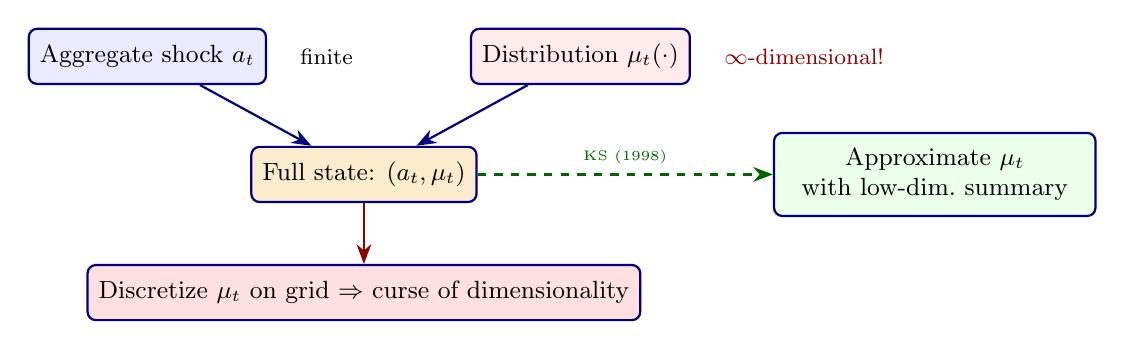
\begin{tikzpicture}[
    box/.style={rectangle, draw=uzhblue, thick, fill=uzhgreylight,
        minimum width=2.5cm, minimum height=0.7cm, font=\small,
        rounded corners=3pt, inner sep=4pt},
    arr/.style={-{Stealth[length=2.5mm]}, thick, uzhblue}
]
    % State components
    \node[box, fill=blue!8] (agg) at (0,0) {Aggregate shock $a_t$};
    \node[box, fill=red!8] (dist) at (5.5,0) {Distribution $\mu_t(\cdot)$};
    \node[box, fill=softorange!20] (state) at (2.75,-1.5) {Full state: $(a_t, \mu_t)$};

    \draw[arr] (agg) -- (state);
    \draw[arr] (dist) -- (state);

    \node[right=0.3cm, font=\small] at (agg.east) {\footnotesize finite};
    \node[right=0.3cm, font=\small, darkred] at (dist.east) {\footnotesize $\infty$-dimensional!};

    % Curse
    \node[box, fill=red!12] (curse) at (2.75,-3.0)
        {Discretize $\mu_t$ on grid $\Rightarrow$ curse of dimensionality};
    \draw[arr, darkred] (state) -- (curse);

    % Solution
    \node[box, fill=green!8] (sol) at (10,-1.5)
        {\begin{tabular}{c}\small Approximate $\mu_t$ \\ \small with low-dim.\ summary\end{tabular}};
    \draw[arr, darkgreen, dashed] (state) -- (sol) node[midway, above, font=\tiny] {KS (1998)};
\end{tikzpicture}
\end{center}

\vspace{0.3em}
\begin{itemize}
    \item Traditional methods: discretize the distribution $\Rightarrow$ exponential cost
    \item Key insight (Krusell--Smith): low-order moments may \emphc{suffice}
\end{itemize}
\end{frame}

% --- Slide 8: Two Approaches ---
\begin{frame}{Two Approaches to Heterogeneous Agents}
\footnotesize
\begin{columns}[T]
\column{0.48\textwidth}
\begin{block}{Approach 1: Finitely Many Agents}
Track $N$ agents explicitly: $(k_1, \ldots, k_N, \varepsilon_1, \ldots, \varepsilon_N)$

\vspace{0.2em}
\textbf{Pro:}
\begin{itemize}\itemsep0pt
    \item Exact---no approximation of $\mu_t$
\end{itemize}

\textbf{Con:}
\begin{itemize}\itemsep0pt
    \item \emphc{Permutation problem}: agents are exchangeable
    \item State space grows with $N$
    \item Scales poorly for large $N$
\end{itemize}

{\scriptsize Maliar, Maliar \& Valli (2010)}
\end{block}

\column{0.48\textwidth}
\begin{block}{Approach 2: Continuum of Agents}
Track the \emphc{distribution} $\mu_t$ directly

\vspace{0.2em}
\textbf{Pro:}
\begin{itemize}\itemsep0pt
    \item Law of large numbers $\Rightarrow$ no sampling noise
    \item No permutation issue
    \item Distribution is order-invariant
\end{itemize}

\textbf{Con:}
\begin{itemize}\itemsep0pt
    \item Must approximate $\mu_t$ (infinite-dimensional)
\end{itemize}

{\scriptsize Krusell \& Smith (1998), Young (2010)}
\end{block}
\end{columns}

\vspace{0.05em}
\begin{center}
{\footnotesize $\Rightarrow$ \textbf{This lecture:} Approach 2 with Young's histogram method + DEQNs.}
\end{center}
\end{frame}

% --- Slide 9: The Krusell-Smith Insight ---
\begin{frame}{The Krusell--Smith Insight (1998)}
\textbf{Key insight:} the \emphc{mean} of the wealth distribution is \emph{nearly sufficient} to predict future prices.

\vspace{0.5em}
\textbf{Approximate bounded rationality:} agents forecast using $m_1 = \int k \, d\mu$ (mean capital).

\vspace{0.5em}
\textbf{Log-linear forecasting rule:}
\[
\boxed{\hat{H}(m_1, a) = \exp\!\bigl(A(a) + B(a) \log m_1\bigr)}
\]

\vspace{0.3em}
\begin{itemize}
    \item Coefficients $A(a), B(a)$ depend on the aggregate shock $a$
    \item Inada conditions ensure capital remains positive and logs are well-defined
    \item $R^2 > 0.999$ in practice---remarkably accurate!
\end{itemize}

\vspace{0.3em}
{\small But \emphc{how do we simulate} the distribution forward to compute realized $m_1$?}
\end{frame}

% --- Slide 9b: Why the Mean Is (Nearly) Sufficient ---
\begin{frame}{Why the Mean Is (Nearly) Sufficient}
\begin{center}
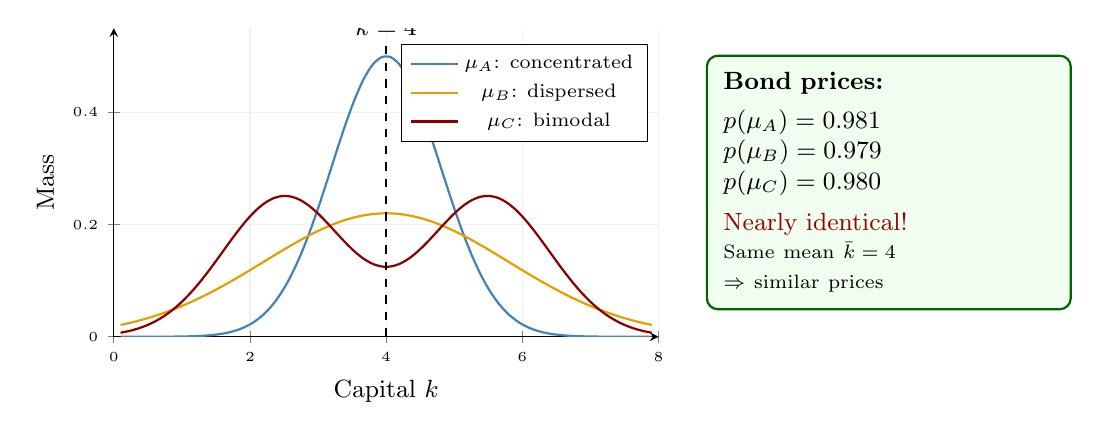
\begin{tikzpicture}
% --- Left: three different distributions with same mean ---
\begin{axis}[
    name=distplot,
    width=8.5cm, height=5.5cm,
    xlabel={Capital $k$},
    ylabel={Mass},
    xlabel style={font=\small},
    ylabel style={font=\small},
    tick label style={font=\tiny},
    xmin=0, xmax=8, ymin=0, ymax=0.55,
    axis lines=left,
    grid=major, grid style={gray!12},
    legend style={font=\scriptsize, at={(0.98,0.95)}, anchor=north east},
]
    % Distribution A: concentrated (low variance)
    \addplot[thick, softblue, smooth, domain=0.1:7.9, samples=60]
        {0.5*exp(-0.5*((x-4)/0.8)^2)};
    \addlegendentry{$\mu_A$: concentrated}
    % Distribution B: spread out (high variance)
    \addplot[thick, softorange, smooth, domain=0.1:7.9, samples=60]
        {0.22*exp(-0.5*((x-4)/1.8)^2)};
    \addlegendentry{$\mu_B$: dispersed}
    % Distribution C: bimodal
    \addplot[thick, darkred, smooth, domain=0.1:7.9, samples=60]
        {0.25*exp(-0.5*((x-2.5)/0.9)^2) + 0.25*exp(-0.5*((x-5.5)/0.9)^2)};
    \addlegendentry{$\mu_C$: bimodal}
    % Mean line
    \draw[thick, black, dashed] (axis cs:4,0) -- (axis cs:4,0.52);
    \node[font=\small, above] at (axis cs:4,0.52) {$\bar{k}=4$};
\end{axis}

% --- Right: price annotation ---
\node[draw=darkgreen, thick, fill=green!6, rounded corners=4pt,
    inner sep=6pt, font=\small, text width=4.2cm, align=left,
    right=0.6cm] at (distplot.east) {
    \textbf{Bond prices:}\\[3pt]
    $p(\mu_A) = 0.981$\\
    $p(\mu_B) = 0.979$\\
    $p(\mu_C) = 0.980$\\[4pt]
    \emphc{Nearly identical!}\\[2pt]
    {\scriptsize Same mean $\bar{k}=4$\\$\Rightarrow$ similar prices}
};
\end{tikzpicture}
\end{center}

\vspace{0.2em}
{\small Three very different distributions that share the same mean capital $\bar{k}=4$.  In the KS economy, the resulting bond prices differ by $< 0.3\%$.  This is why the mean is a nearly sufficient statistic for forecasting---and why \emphc{approximate aggregation} works so well.}
\end{frame}

% --- Slide 10: But How Do We Simulate the Distribution? ---
\begin{frame}{But How Do We Simulate the Distribution?}
Given policy functions, need to compute the next-period distribution $\mu_{t+1}$.

\vspace{0.5em}
\begin{columns}[T]
\column{0.48\textwidth}
\textbf{Option A: Monte Carlo simulation}
\begin{itemize}
    \item Draw $N$ agents, simulate forward, compute sample moments
    \item Problem: \emphc{sampling noise} $\sim O(1/\sqrt{N})$
    \item Need very large $N$ ($> 50{,}000$) for accurate means
    \item Noise accumulates over time
\end{itemize}

\column{0.48\textwidth}
\textbf{Option B: Non-stochastic simulation}\\
{\small (Young, 2010)}
\begin{itemize}
    \item Track the \emphc{histogram} directly on a fixed grid
    \item \emphc{No sampling error}---deterministic update
    \item Preserves the mean \emphc{exactly}
    \item Computationally fast
\end{itemize}
\end{columns}

\vspace{0.5em}
\begin{center}
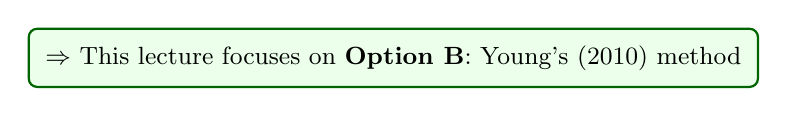
\begin{tikzpicture}
    \node[rectangle, draw=darkgreen, thick, fill=green!8, rounded corners=3pt,
        inner sep=6pt, font=\small] {$\Rightarrow$ This lecture focuses on \textbf{Option B}: Young's (2010) method};
\end{tikzpicture}
\end{center}
\end{frame}

% --- Slide 11: Roadmap Reminder ---
\begin{frame}{Where Are We?}
\begin{enumerate}
    \item \textcolor{gray}{Motivation: Why Track Distributions?} \checkmark
    \vspace{0.25em}
    \item \emphc{$\Rightarrow$ Young's (2010) Non-Stochastic Simulation}
    \vspace{0.25em}
    \item \textcolor{gray}{Benchmark: Krusell--Smith (1998)}
    \vspace{0.25em}
    \item \textcolor{gray}{DEQN teaching implementation}
    \vspace{0.25em}
    \item \textcolor{gray}{Alternative deep-learning approaches to KS}
\end{enumerate}
\end{frame}

% ============================================================================
% PART II: YOUNG'S METHOD
% ============================================================================

% --- Slide 12: Section Divider ---
\begin{frame}{}
\vfill
\begin{center}
{\Huge \textcolor{uzhblue}{\textbf{Part II}}}\\[12pt]
{\LARGE Young's (2010) Non-Stochastic Simulation}
\end{center}
\vfill
\end{frame}

% --- Slide 13: The Core Idea ---
\begin{frame}{The Core Idea}
Instead of simulating a \emphc{panel of agents} $\longrightarrow$ simulate the \emphc{distribution} directly.

\vspace{0.5em}
\textbf{Setup:}
\begin{enumerate}
    \item Choose a \emphc{fixed grid}: $[w_1, w_2, \ldots, w_N]$
    \item Represent the distribution as a \emphc{histogram}: mass $G(w_i)$ at each grid point
    \item Update the histogram \emphc{deterministically} using:
    \begin{itemize}
        \item Policy functions $k' = g(k, \varepsilon, m_1, a)$
        \item Transition probabilities $\pi_{\varepsilon' | \varepsilon, a}$
    \end{itemize}
\end{enumerate}

\vspace{0.5em}
\begin{block}{Key insight}
When $k'$ falls between grid points, \emphc{redistribute the mass} to the two nearest grid points using linear interpolation weights. This preserves the mean exactly.
\end{block}
\end{frame}

% --- Slide 14: Mass Redistribution: Single Point ---
\begin{frame}{Mass Redistribution: The Key Operation}
\begin{center}
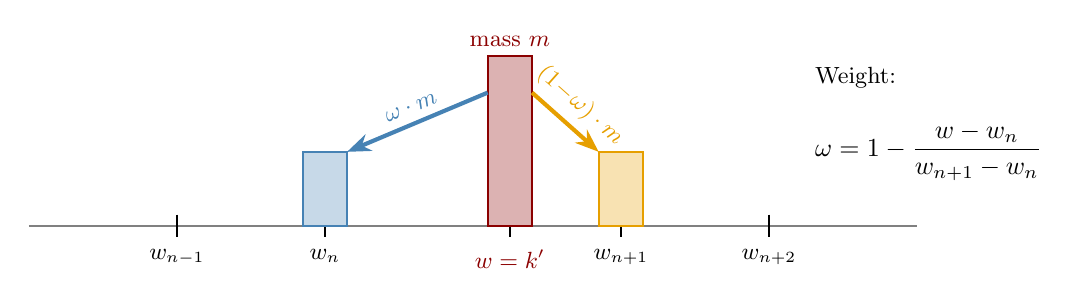
\begin{tikzpicture}[scale=0.94, every node/.style={transform shape}]
    % Grid line
    \draw[thick, gray] (0,0) -- (12,0);

    % Grid points
    \foreach \x/\lab in {2/$w_{n-1}$, 4/$w_n$, 6.5/$w$, 8/$w_{n+1}$, 10/$w_{n+2}$} {
        \draw[thick] (\x,0.15) -- (\x,-0.15);
    }
    \node[below, font=\small] at (2,-0.2) {$w_{n-1}$};
    \node[below, font=\small] at (4,-0.2) {$w_n$};
    \node[below, font=\small, darkred] at (6.5,-0.2) {$w = k'$};
    \node[below, font=\small] at (8,-0.2) {$w_{n+1}$};
    \node[below, font=\small] at (10,-0.2) {$w_{n+2}$};

    % Mass at w
    \draw[thick, darkred, fill=darkred!30] (6.2,0) rectangle (6.8,2.3);
    \node[above, font=\small, darkred] at (6.5,2.3) {mass $m$};

    % Arrows
    \draw[-{Stealth[length=3mm]}, thick, softblue, line width=1.5pt]
        (6.2,1.8) -- (4.3,1.0) node[midway, above, font=\small, sloped] {$\omega \cdot m$};
    \draw[-{Stealth[length=3mm]}, thick, softorange, line width=1.5pt]
        (6.8,1.8) -- (7.7,1.0) node[midway, above, font=\small, sloped] {$(1\!-\!\omega) \cdot m$};

    % Result bars
    \draw[thick, softblue, fill=softblue!30] (3.7,0) rectangle (4.3,1.0);
    \draw[thick, softorange, fill=softorange!30] (7.7,0) rectangle (8.3,1.0);

    % Formula
    \node[right, font=\small] at (10.5,2.0) {Weight:};
    \node[right] at (10.5,1.0) {$\displaystyle \omega = 1 - \frac{w - w_n}{w_{n+1} - w_n}$};
\end{tikzpicture}
\end{center}

\vspace{-0.2em}
\begin{itemize}\footnotesize
    \setlength{\itemsep}{0pt}
    \item Mass $m$ at $w \in [w_n, w_{n+1}]$ is split between the two bracketing grid points
    \item Weight $\omega$: fraction to $w_n$ (closer $\Rightarrow$ more mass)
    \item Weight $1-\omega$: fraction to $w_{n+1}$
\end{itemize}
\end{frame}

% --- Slide 14b (NEW): Lottery view ---
\begin{frame}{Lottery View: Why ``Non-Stochastic''}
\small
\begin{block}{The redistribution \emph{is} a lottery}
Every agent at $(k, \varepsilon)$ whose policy choice $k'$ lands between $k_n$ and $k_{n+1}$ is reassigned by a \emphc{biased coin}:
\[
k_{t+1} = \begin{cases} k_n     & \text{with probability } \omega,\\ k_{n+1} & \text{with probability } 1-\omega,\end{cases}
\qquad \omega = 1 - \frac{k' - k_n}{k_{n+1} - k_n}.
\]
\end{block}

\begin{columns}[T]
\column{0.49\textwidth}
\textbf{Monte Carlo panel}\\[2pt]
Each of $N$ agents \emphc{draws the lottery once}.\\
Empirical histogram converges at rate $\mathcal{O}(N^{-1/2})$.\\
Sampling noise contaminates aggregates.
\column{0.49\textwidth}
\textbf{Young's method}\\[2pt]
\emphc{Integrates the lottery analytically.}\\
Equivalent to running $N = \infty$ agents.\\
Zero noise; mean preserved exactly.
\end{columns}

\vspace{0.2em}
{\footnotesize The same trick is applied to the shock transitions $\pi_{\varepsilon\varepsilon'}$: each piece of mass goes into \emph{all} reachable next-period $\varepsilon'$ in proportion to $\pi$, instead of one realisation being drawn.}
\end{frame}

% --- Slide 14c (NEW): Cascading fork ---
\begin{frame}{One Cell Splits Into Four (Young, Fig.~1)}
\small
\centering
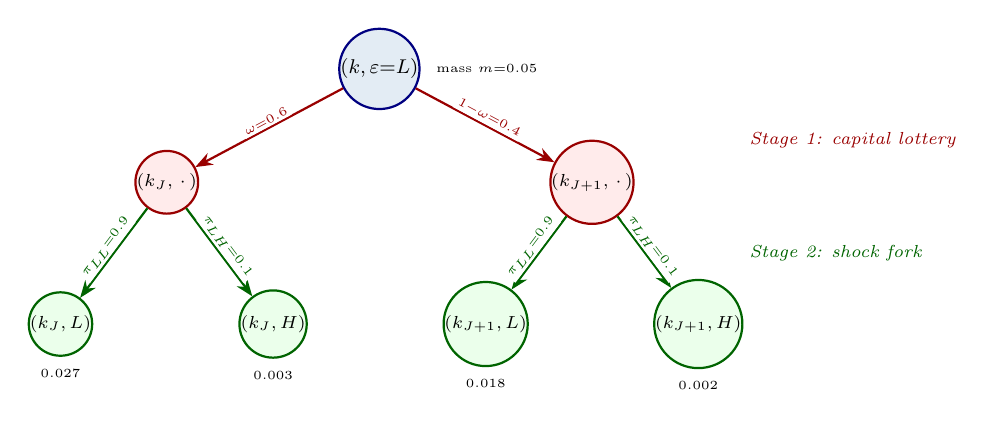
\begin{tikzpicture}[scale=0.9, every node/.style={transform shape},
    src/.style={circle, draw=uzhblue, thick, fill=softblue!15,
        minimum size=0.95cm, font=\footnotesize, inner sep=0pt},
    mid/.style={circle, draw=harvardcrimson, thick, fill=red!8,
        minimum size=0.85cm, font=\scriptsize, inner sep=0pt},
    leaf/.style={circle, draw=darkgreen, thick, fill=green!8,
        minimum size=0.85cm, font=\scriptsize, inner sep=0pt},
    arr/.style={-{Stealth[length=2.2mm]}, thick},
    lab/.style={font=\tiny, midway, fill=white, inner sep=1pt}
]
    \node[src] (S) at (0,3.0) {$(k,\varepsilon{=}L)$};
    \node[font=\tiny, right=0.1cm] at (S.east) {mass $m{=}0.05$};

    \node[mid] (M1) at (-3.0,1.4) {$(k_J,\,\cdot\,)$};
    \node[mid] (M2) at ( 3.0,1.4) {$(k_{J+1},\,\cdot\,)$};

    \node[leaf] (L1) at (-4.5,-0.6) {$(k_J,L)$};
    \node[leaf] (L2) at (-1.5,-0.6) {$(k_J,H)$};
    \node[leaf] (L3) at ( 1.5,-0.6) {$(k_{J{+}1},L)$};
    \node[leaf] (L4) at ( 4.5,-0.6) {$(k_{J{+}1},H)$};

    \draw[arr, harvardcrimson] (S) -- (M1) node[lab, above, sloped] {$\omega{=}0.6$};
    \draw[arr, harvardcrimson] (S) -- (M2) node[lab, above, sloped] {$1{-}\omega{=}0.4$};

    \draw[arr, darkgreen] (M1) -- (L1) node[lab, above, sloped] {$\pi_{LL}{=}0.9$};
    \draw[arr, darkgreen] (M1) -- (L2) node[lab, above, sloped] {$\pi_{LH}{=}0.1$};
    \draw[arr, darkgreen] (M2) -- (L3) node[lab, above, sloped] {$\pi_{LL}{=}0.9$};
    \draw[arr, darkgreen] (M2) -- (L4) node[lab, above, sloped] {$\pi_{LH}{=}0.1$};

    \node[font=\tiny, below=0.05cm] at (L1.south) {$0.027$};
    \node[font=\tiny, below=0.05cm] at (L2.south) {$0.003$};
    \node[font=\tiny, below=0.05cm] at (L3.south) {$0.018$};
    \node[font=\tiny, below=0.05cm] at (L4.south) {$0.002$};

    \node[font=\scriptsize\itshape, harvardcrimson, anchor=west] at (5.1,2.0) {Stage 1: capital lottery};
    \node[font=\scriptsize\itshape, darkgreen,    anchor=west] at (5.1,0.4) {Stage 2: shock fork};
\end{tikzpicture}

\vspace{0.2em}
{\footnotesize Verification: $0.027 + 0.003 + 0.018 + 0.002 = 0.05 = m$ \emphc{$\checkmark$}.\quad Repeat for every active source bin and accumulate the leaves to obtain $G_{t+1}$.}
\end{frame}

% --- Slide 16: Visual Example: Multi-Point Distribution ---
\begin{frame}{Example: Multi-Point Distribution}
\begin{columns}[T]
\column{0.48\textwidth}
\begin{center}
\textbf{True distribution}\\[2pt]
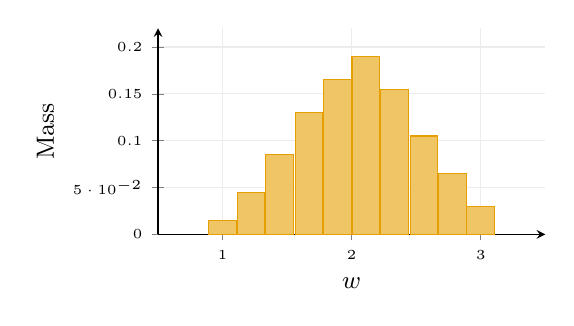
\begin{tikzpicture}
\begin{axis}[
    width=6.5cm, height=4.2cm,
    ybar, bar width=10pt,
    xlabel={$w$}, ylabel={Mass},
    xlabel style={font=\small},
    ylabel style={font=\small},
    tick label style={font=\tiny},
    xmin=0.5, xmax=3.5,
    ymin=0, ymax=0.22,
    grid=major, grid style={gray!15},
    axis lines=left,
]
    \addplot[fill=softorange!60, draw=softorange] coordinates {
        (1.0,0.015) (1.22,0.045) (1.44,0.085) (1.67,0.13) (1.89,0.165)
        (2.11,0.19) (2.33,0.155) (2.56,0.105) (2.78,0.065) (3.0,0.03)
    };
\end{axis}
\end{tikzpicture}\\
{\tiny 10 points with truncated normal masses}
\end{center}

\column{0.48\textwidth}
\begin{center}
\textbf{Histogram approximation}\\[2pt]
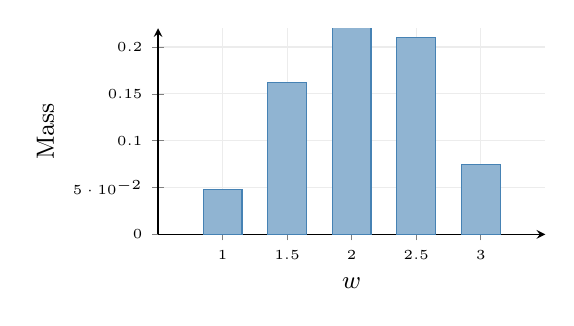
\begin{tikzpicture}
\begin{axis}[
    width=6.5cm, height=4.2cm,
    ybar, bar width=14pt,
    xlabel={$w$}, ylabel={Mass},
    xlabel style={font=\small},
    ylabel style={font=\small},
    tick label style={font=\tiny},
    xmin=0.5, xmax=3.5,
    ymin=0, ymax=0.22,
    xtick={1.0,1.5,2.0,2.5,3.0},
    grid=major, grid style={gray!15},
    axis lines=left,
]
    \addplot[fill=softblue!60, draw=softblue] coordinates {
        (1.0,0.048) (1.5,0.162) (2.0,0.28) (2.5,0.21) (3.0,0.075)
    };
\end{axis}
\end{tikzpicture}\\
{\tiny 5-point grid approximation}
\end{center}
\end{columns}

\vspace{0.05em}
\begin{center}
\footnotesize
\begin{tabular}{@{}lcc@{}}
\toprule
& \textbf{True} & \textbf{Approximation} \\
\midrule
Mean & 2.0 & \emphc{2.0 (exact!)} \\
Variance & 0.347 & 0.384 (approx.) \\
\bottomrule
\end{tabular}
\end{center}
\end{frame}

% --- Slide 17: Key Property: Mean Preservation ---
\begin{frame}{Key Property: Mean Preservation}
\small
\begin{block}{The weight $\omega$ is forced by mean preservation}
$\omega$ is the \emphc{unique} value for which the two-point split $\{\omega \cdot w_n,\, (1-\omega)\cdot w_{n+1}\}$ has expected value equal to the off-grid policy $w$.  Solving $\omega\cdot w_n + (1-\omega)\cdot w_{n+1} = w$ for $\omega$ gives back $\omega = 1 - (w-w_n)/(w_{n+1}-w_n)$ in one line:
\[
\omega\cdot w_n + (1-\omega)\cdot w_{n+1} \;=\; w_n + (1-\omega)(w_{n+1}-w_n) \;=\; w_n + (w-w_n) \;=\; w. \quad\checkmark
\]
\end{block}

\vspace{0.2em}
\begin{itemize}\itemsep1pt
    \item Total mass preserved automatically: $\omega + (1-\omega) = 1$.
    \item By linearity of expectation, the unconditional mean of $G_{t+1}$ equals $\mathbb{E}[k']$ \emph{exactly}, provided no mass leaks past the grid endpoints.
\end{itemize}

\vspace{0.2em}
\begin{alertblock}{Caution}
\emphc{Higher moments} (variance, percentiles) are only \emph{approximated}---finer grid $=$ better approximation. Linear interpolation is exact for linear functions but smooths nonlinear ones.
\end{alertblock}
\end{frame}

% --- Slide 18a: Why Not Just Use a Panel? (table) ---
\begin{frame}{Why Not Just Use a Panel?}
\small
\begin{center}
\begin{tabular}{@{}lcc@{}}
\toprule
& \textbf{Young's Method} & \textbf{Panel Simulation} \\
\midrule
Sampling noise & \emphc{None} & $O(1/\sqrt{N})$ \\
Mean preservation & \emphc{Exact} & Approximate \\
Agents/points needed & $\sim$100--5000 grid pts & $>$50,000 agents \\
Speed & \emphc{Fast} (deterministic) & Slower (stochastic) \\
Memory & Fixed grid & Growing with $N$ \\
Reproducibility & \emphc{Deterministic} & Seed-dependent \\
\bottomrule
\end{tabular}
\end{center}

\vspace{0.6em}
\begin{itemize}\footnotesize\itemsep2pt
    \item \emphc{Mean preservation} is the headline property: each Young update reassigns mass deterministically using the lottery weight $\omega$, so the new mean equals the policy-implied mean exactly (boundary clipping aside).
    \item In a Monte-Carlo panel the same lottery is \emph{drawn once per agent}, so the realized mean is noisy at rate $1/\sqrt{N}$.
\end{itemize}

\vspace{0.3em}
{\footnotesize $\Rightarrow$ The next slide quantifies the gap.}
\end{frame}

% --- Slide 18b: Convergence plot with interpretation ---
\begin{frame}{Convergence: Young vs.\ Monte-Carlo Panel}
\vspace{-0.2em}
\begin{center}
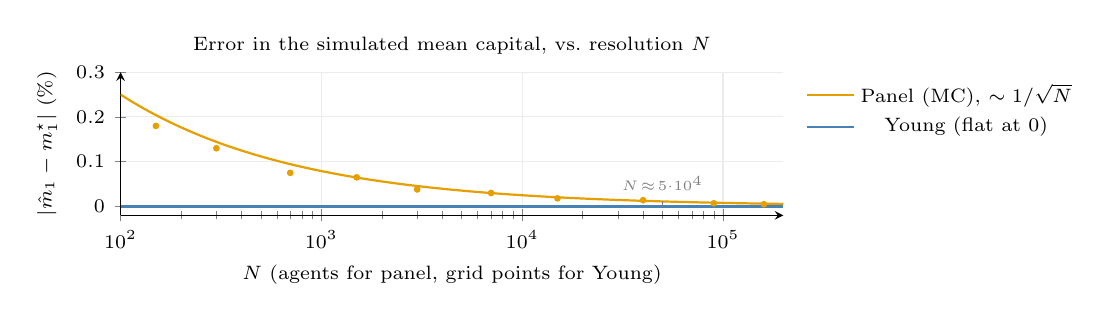
\begin{tikzpicture}
\begin{axis}[
    width=10.0cm, height=3.4cm,
    title={\scriptsize Error in the simulated mean capital, vs.\ resolution $N$},
    title style={font=\scriptsize, yshift=-3pt},
    xlabel={$N$ (agents for panel, grid points for Young)},
    ylabel={$|\hat{m}_1 - m_1^\star|$ (\%)},
    xlabel style={font=\scriptsize, yshift=1pt},
    ylabel style={font=\scriptsize},
    tick label style={font=\scriptsize},
    xmode=log,
    xmin=100, xmax=200000,
    ymin=-0.02, ymax=0.30,
    ytick={0,0.1,0.2,0.3},
    grid=major, grid style={gray!15},
    legend style={font=\scriptsize, draw=none, fill=none,
                  at={(1.02,1.0)}, anchor=north west},
    axis lines=left,
]
    % Panel simulation: O(1/sqrt(N)) envelope (smooth decay)
    \addplot[thick, softorange, domain=100:200000, samples=60, smooth]
        {2.5/sqrt(x)};
    \addlegendentry{Panel (MC), $\sim 1/\sqrt{N}$}
    % Scatter points: sampled MC errors jittered around the envelope
    \addplot[only marks, mark=*, mark size=1pt, softorange, forget plot]
        coordinates {
            (150,0.18) (300,0.13) (700,0.075) (1500,0.065)
            (3000,0.038) (7000,0.030) (15000,0.018) (40000,0.014)
            (90000,0.007) (160000,0.005)
        };
    % Young's method: zero deviation
    \addplot[thick, softblue, domain=100:200000, samples=2] {0};
    \addlegendentry{Young (flat at $0$)}
    % Annotation: pin the matching-accuracy point
    \draw[gray, dashed, thin] (axis cs:50000,0) -- (axis cs:50000,0.012);
    \node[font=\tiny, gray, anchor=south] at (axis cs:50000,0.012) {$N\!\approx\!5{\cdot}10^4$};
\end{axis}
\end{tikzpicture}
\end{center}

\vspace{0.1em}
{\scriptsize\textbf{What is plotted.} Deviation of the simulated mean capital $\hat{m}_1$ from its true value $m_1^\star$, as the resolution $N$ grows. \emphc{Orange dots}: realized Monte-Carlo errors of a panel of $N$ agents, scattered around the $1/\sqrt{N}$ envelope. \emphc{Blue line}: Young's deterministic update, which preserves the mean exactly at \emph{every} grid resolution.\\[2pt]
\textbf{Implication.} To match Young's accuracy at $\sim\!1{,}000$ grid points, a Monte-Carlo panel needs $\gtrsim 50{,}000$ agents (an order of magnitude more state), and the residual noise still contaminates the OLS step that updates the KS forecasting rule.}
\end{frame}

% --- Slide 19: The Algorithm: Setup ---
\begin{frame}{The Algorithm: Setup}
\textbf{Ingredients:}
\begin{itemize}
    \item \textbf{Asset grid:} $[k_1, k_2, \ldots, k_{N_k}]$ for individual capital/asset holdings
    \item \textbf{Idiosyncratic states:} $\varepsilon \in \{e, u\}$ (employed/unemployed)
    \item \textbf{Histogram:} $G_t(k_i, \varepsilon_j) =$ mass of agents at grid point $k_i$ with shock $\varepsilon_j$
    \item \textbf{Total bins:} $N_k \times N_\varepsilon$ histogram entries
\end{itemize}

\vspace{0.5em}
\textbf{Normalization:}
\[
\sum_{i=1}^{N_k} \sum_{j=1}^{N_\varepsilon} G_t(k_i, \varepsilon_j) = 1
\]

\vspace{0.3em}
\textbf{First moment (mean capital):}
\[
m_1 = \sum_{i=1}^{N_k} \sum_{j=1}^{N_\varepsilon} G_t(k_i, \varepsilon_j) \cdot k_i
\]
\end{frame}

% --- Slide 20: The Algorithm: One Forward Step ---
\begin{frame}{The Algorithm: One Forward Step}
\begin{block}{Algorithm: Histogram Update at Time $t$}
\begin{algorithmic}
\footnotesize
\STATE \textbf{Input:} Current histogram $G_t$, policy $g(\cdot)$, transition $\pi_{\varepsilon'|\varepsilon,a}$, grid $\{k_j\}$
\STATE Initialize $G_{t+1}(k_j, \varepsilon') = 0$ for all $(j, \varepsilon')$
\FOR{each $(k_i, \varepsilon_j)$ with $G_t(k_i, \varepsilon_j) > 0$}
    \STATE Compute optimal savings: $k' = g(k_i, \varepsilon_j, m_1, a_t)$
    \STATE Find bracketing grid points: $k' \in [k_J, k_{J+1}]$
    \STATE Compute lottery weight: $\omega = 1 - \frac{k' - k_J}{k_{J+1} - k_J}$
    \FOR{each next-period shock $\varepsilon'$}
        \STATE $G_{t+1}(k_J, \varepsilon') ~\mathrel{+}=~ \omega \cdot \pi_{\varepsilon'|\varepsilon_j, a_t} \cdot G_t(k_i, \varepsilon_j)$
        \STATE $G_{t+1}(k_{J+1}, \varepsilon') ~\mathrel{+}=~ (1\!-\!\omega) \cdot \pi_{\varepsilon'|\varepsilon_j, a_t} \cdot G_t(k_i, \varepsilon_j)$
    \ENDFOR
\ENDFOR
\STATE \textbf{Output:} Updated histogram $G_{t+1}$
\end{algorithmic}
\end{block}

\vspace{-0.3em}
{\scriptsize \emphc{Notation note.}  The interpolation weight is denoted $\omega$ throughout this deck and the script.  It is the probability mass sent to the lower bracketing grid point.}
\end{frame}

% --- Slide 20b (NEW): Implementation cheatsheet ---
\begin{frame}[fragile]{Implementation: Young's Update in NumPy}
\footnotesize
Four scatter-add lines (one per leaf of the cascading fork):

\begin{lstlisting}[language=Python, basicstyle=\tiny\ttfamily, frame=single, backgroundcolor=\color{uzhgreylight}, numbers=none, aboveskip=2pt, belowskip=2pt]
def young_step(G, kp, pi_eps, k_grid):
    """G[i,j]: mass at (k_grid[i], eps_j); kp[i,j]: policy k'."""
    G_next = np.zeros_like(G)
    dk     = k_grid[1] - k_grid[0]
    n_k    = len(k_grid)
    for j in range(G.shape[1]):
        for i in range(G.shape[0]):
            x     = np.clip(kp[i, j], k_grid[0], k_grid[-1])
            J     = min(int((x - k_grid[0]) // dk), n_k - 2)
            omega = (k_grid[J + 1] - x) / dk            # in [0, 1]
            for jp in range(G.shape[1]):
                w = pi_eps[j, jp] * G[i, j]
                G_next[J,     jp] += omega       * w
                G_next[J + 1, jp] += (1 - omega) * w
    return G_next
\end{lstlisting}

\vspace{0.1em}
{\scriptsize JAX vectorisation of the same operator (\texttt{distribution\_step} via \texttt{jax.vmap} and \texttt{.at[].add()}) is in \texttt{KrusellSmith\_Tutorial\_CPU.ipynb}.}
\end{frame}

% --- Slide 20c (NEW): GPU bracketing motivation ---
\begin{frame}{Why Closed-Form Bracketing Matters on GPUs}
\footnotesize
\textbf{The lookup.}  Young's update --- and any piecewise-linear interpolation --- needs the bracketing index for each query $k'$:
\[
  J(k') \;=\; \max\{\,n : k_n \le k'\,\},\qquad k' \in [k_J,\, k_{J+1}).
\]

\vspace{0.4em}
\textbf{Generic approach.}  Binary search (e.g.\ \texttt{jnp.searchsorted}): $\mathcal{O}(\log N_k)$ per query, with data-dependent branches.

\vspace{0.4em}
\textbf{Consequences on GPU / under XLA.}
\begin{itemize}\itemsep1pt
  \item \emphc{Warp divergence} across SIMT threads taking different branches.
  \item Irregular gather patterns and extra kernel launches.
  \item Opaque search op breaks fusion with the surrounding interpolation arithmetic.
\end{itemize}

\vspace{0.4em}
\textbf{Closed-form alternative (uniform grid).}
\[
  J(k') \;=\; \mathrm{clip}\!\left(\Big\lfloor \tfrac{k' - k_0}{\Delta k}\Big\rfloor,\;0,\;N_k-2\right).
\]
\emphc{One fused multiply--add and a cast}: branch-free, uniform across threads, fuses with the lottery weight $\omega = (k_{J+1}-k')/\Delta k$ into a single GPU kernel.  This is exactly the line \texttt{J = int((x - k\_grid[0]) // dk)} on the previous slide.
\end{frame}

% --- Slide 20d (NEW): Log-spaced grids ---
\begin{frame}{Log-Spaced Grids Without Giving Up the Closed Form}
\footnotesize
\textbf{Why log-spacing.}  The consumption policy is steepest near the borrowing constraint $k\!\to\!0$; we want fine resolution there without wasting points in the right tail.

\vspace{0.4em}
\textbf{Recipe.}  Equidistant knots in a transformed coordinate $x = \log(c+k)$ for a small shift $c>0$:
\[
  x_n \,=\, x_0 + n\,\Delta x,\qquad k_n \,=\, e^{x_n} - c,\qquad n=0,\dots,N_k.
\]

\vspace{0.4em}
\textbf{Bracketing stays closed-form.}
\[
  J(k') \;=\; \mathrm{clip}\!\left(\Big\lfloor \tfrac{\log(c+k') - x_0}{\Delta x}\Big\rfloor,\;0,\;N_k-2\right).
\]
Still $\mathcal{O}(1)$ per query, no search, no branches.

\vspace{0.4em}
\textbf{Keep interpolation in $k$-space.}  The \emph{index} is computed in $x$-space, but the lottery \emph{weights} use the original $k_n$'s, so the off-grid policy is piecewise linear in $k$ --- consistent with the on-grid consumption values and with Young's mean-preserving lottery.

\vfill
{\scriptsize Concrete implementation: \texttt{interpolate()} and \texttt{distribution\_step()} in the Krusell--Smith JAX tutorial of Azinovic-Yang \& \v{Z}emli\v{c}ka (2025), \emph{Deep Learning in the Sequence Space}, \href{https://arxiv.org/abs/2509.13623}{arXiv:2509.13623}.}
\end{frame}

% --- Slide 21: TikZ Flow Diagram ---
\begin{frame}{Flow Diagram: One Forward Step}
\begin{center}
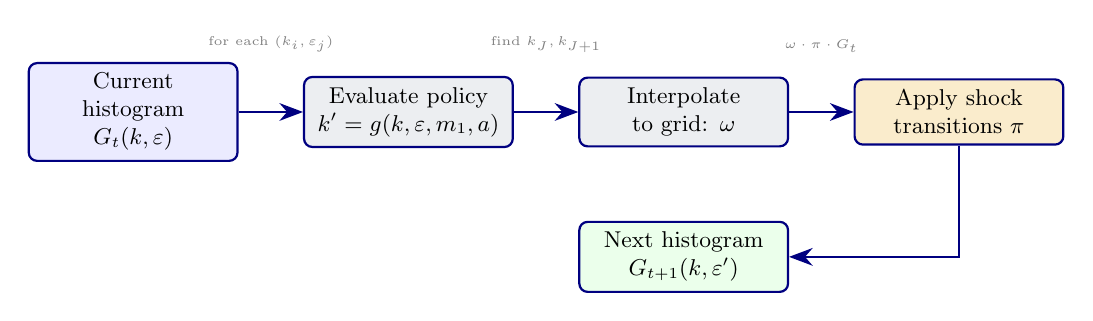
\begin{tikzpicture}[scale=0.92, every node/.style={transform shape},
    box/.style={rectangle, draw=uzhblue, thick, fill=uzhgreylight,
        minimum width=2.8cm, minimum height=0.9cm, font=\small,
        rounded corners=3pt, inner sep=4pt, text width=2.6cm, align=center},
    arr/.style={-{Stealth[length=3mm]}, thick, uzhblue}
]
    \node[box, fill=blue!8] (hist) at (0,0) {Current histogram\\$G_t(k,\varepsilon)$};
    \node[box] (pol) at (3.8,0) {Evaluate policy\\$k' = g(k,\varepsilon,m_1,a)$};
    \node[box] (interp) at (7.6,0) {Interpolate\\to grid: $\omega$};
    \node[box, fill=softorange!20] (trans) at (11.4,0) {Apply shock\\transitions $\pi$};
    \node[box, fill=green!8] (next) at (7.6,-2) {Next histogram\\$G_{t+1}(k,\varepsilon')$};

    \draw[arr] (hist) -- (pol);
    \draw[arr] (pol) -- (interp);
    \draw[arr] (interp) -- (trans);
    \draw[arr] (trans) |- (next);

    % Annotations
    \node[font=\tiny, gray, above=0.1cm] at (1.9,0.6) {for each $(k_i,\varepsilon_j)$};
    \node[font=\tiny, gray, above=0.1cm] at (5.7,0.6) {find $k_J, k_{J+1}$};
    \node[font=\tiny, gray, above=0.1cm] at (9.5,0.6) {$\omega \cdot \pi \cdot G_t$};
\end{tikzpicture}
\end{center}

\vspace{0.1em}
\textbf{Key properties of each step:}
\begin{itemize}\footnotesize
    \setlength{\itemsep}{1pt}
    \item \textbf{Policy evaluation}: uses the solution from value function iteration (or neural net)
    \item \textbf{Interpolation}: linear weights ensure mean preservation
    \item \textbf{Shock transition}: probability-weighted mass redistribution across $\varepsilon'$ states
    \item \textbf{Result}: $G_{t+1}$ sums to 1 and has the policy-implied mean. At the fixed point this matches $\hat{H}(m_1,a)$; away from it, the outer loop closes the gap.
\end{itemize}
\end{frame}

% --- Slide 22: The Full Algorithm ---
\begin{frame}{The Full Algorithm: Iterating to Equilibrium}
\begin{block}{Krusell--Smith Algorithm with Young's Simulation}
\begin{algorithmic}
\footnotesize
\STATE \textbf{Step 1:} Initialize forecasting coefficients $A(a), B(a)$
\REPEAT
    \STATE \textbf{Step 2:} Solve household problem via VFI given forecasting rule $\hat{H}$
    \STATE \textbf{Step 3:} Forward-simulate distribution for $T$ periods via Young's method:
    \FOR{$t = 1, \ldots, T$}
        \STATE Draw aggregate shock $a_t$ from Markov chain
        \STATE Update histogram: $G_t \xrightarrow{\text{Young}} G_{t+1}$
        \STATE Record realized mean: $m_1^t = \sum_{i,j} G_t(k_i, \varepsilon_j) \cdot k_i$
    \ENDFOR
    \STATE \textbf{Step 4:} Re-estimate $A(a), B(a)$ by OLS on simulated $(m_1^t, m_1^{t+1}, a_t)$
    \STATE \textbf{Step 5:} Check convergence: $|A^{\text{new}} - A^{\text{old}}| < \text{tol}$
\UNTIL{converged}
\end{algorithmic}
\end{block}
\end{frame}

% --- Finger Exercise: Young's Method ---
\begin{frame}{\exercisepause{} Finger Exercise: Histogram Mass Redistribution}
\begin{exampleblock}{Exercise}
Consider a 4-bin histogram on the grid $\{0.5, 1.0, 1.5, 2.0\}$ with initial masses $\mu = (0.25, 0.25, 0.25, 0.25)$.  Suppose the policy function maps:
\[
g(0.5) = 0.8, \quad g(1.0) = 1.3, \quad g(1.5) = 1.7, \quad g(2.0) = 1.9.
\]
\begin{enumerate}
    \item For $g(0.5) = 0.8$: which two grid points does 0.8 fall between?  What are the interpolation weights?
    \item Compute the updated mass $\mu'$ at grid point $1.0$ after redistributing the mass from $g(0.5) = 0.8$ only (ignoring other bins for now).
\end{enumerate}
\end{exampleblock}
\end{frame}

\begin{frame}{Solution: Histogram Mass Redistribution}
\begin{block}{Answer}
\begin{enumerate}
    \item $g(0.5) = 0.8$ falls between grid points $0.5$ and $1.0$.\\
    Weight on $1.0$: $\omega = \frac{0.8 - 0.5}{1.0 - 0.5} = 0.6$. \quad Weight on $0.5$: $1 - \omega = 0.4$.
    \item The mass $\mu(0.5) = 0.25$ is split: grid point $1.0$ receives $0.6 \times 0.25 = 0.15$, and grid point $0.5$ receives $0.4 \times 0.25 = 0.10$.

    To get the full updated $\mu'(1.0)$, you would also add contributions from any other bins whose policy maps into the $[0.5, 1.5]$ interval---but this exercise only asked for the contribution from $g(0.5)$.
\end{enumerate}
Total mass is preserved: $0.10 + 0.15 = 0.25$ = original mass at bin $0.5$. \checkmark
\end{block}
\end{frame}

% --- Slide 23: Convergence and Accuracy ---
\begin{frame}{Convergence and Accuracy}
\textbf{Quality of the forecasting rule:}
\begin{itemize}
    \item $R^2 > 0.999$ for the log-linear rule $\hat{H}(m_1, a) = \exp(A(a) + B(a) \log m_1)$
    \item KS (1998) also tested 2- and 3-moment rules (adding variance, skewness): $R^2$ barely changes
    \item The one-moment benchmark is an \emphc{empirical finding}, not a modeling restriction
\end{itemize}

\vspace{0.5em}
\textbf{Accuracy tests (Den Haan, 2009):}
\begin{itemize}
    \item Compare simulated $m_1$ path with the forecasting rule prediction
    \item Maximum one-step-ahead forecast error $< 0.1\%$
    \item Simulation length: $T = 10{,}000$ periods (discarding first 500 for burn-in)
\end{itemize}

\vspace{0.5em}
\textbf{Convergence speed:}
\begin{itemize}
    \item Young's non-stochastic simulation removes MC noise from the simulated means
    \item Each iteration still includes VFI + forward simulation + OLS
    \item Outer-loop counts and runtime are tolerance- and implementation-dependent
\end{itemize}
\end{frame}

% --- Slide 24: Implementation: Grid Design ---
\begin{frame}{Implementation: Grid Design}
\textbf{Practical considerations from Young (2010):}

\vspace{0.5em}
\begin{columns}[T]
\column{0.48\textwidth}
\textbf{Value function grid:}
\begin{itemize}
    \item $\sim$150 points, \emphc{irregularly spaced}
    \item Finer near the borrowing constraint (high curvature)
    \item Coarser for large $k$ (smooth policy)
    \item Used for VFI with cubic splines
\end{itemize}

\column{0.48\textwidth}
\textbf{Simulation grid:}
\begin{itemize}
    \item $\sim$5000 points, \emphc{uniformly spaced}
    \item Uniform spacing essential for smooth histograms
    \item Avoids spikes in the distribution
    \item Upper bound: $k_{\max} = 1200$ (large enough)
\end{itemize}
\end{columns}

\vspace{0.5em}
\begin{alertblock}{Important}
\emphc{Two separate grids}: one for solving (irregular, fewer points), one for simulating (uniform, many points). The simulation grid must be fine and uniform to produce smooth distributions.
\end{alertblock}
\end{frame}

% --- Slide 26: Boundary Cases ---
\begin{frame}{Boundary Cases}
\textbf{What happens at the grid boundaries?}

\vspace{0.5em}
\begin{itemize}
    \item $k' \leq k_{\min}$: all mass goes to the \emphc{first grid point} ($p = 1$)
    \item $k' \geq k_{\max}$: all mass goes to the \emphc{last grid point} ($p = 0$)
\end{itemize}

\vspace{0.5em}
\textbf{Importance of grid bounds:}
\begin{itemize}
    \item If $k_{\max}$ is too small, mass ``piles up'' at the boundary $\Rightarrow$ \emphc{mean is not preserved}
    \item If $k_{\max}$ is too large, the grid wastes resolution in empty regions
    \item Rule of thumb: run a preliminary simulation, check that no mass reaches boundaries
\end{itemize}

\vspace{0.5em}
\begin{block}{From the code (Azinovic et al.\ 2022)}
\vspace{-0.2em}
\texttt{anext = tf.minimum(anext, amax * tf.ones\_like(anext))}\\[2pt]
{\small Asset holdings are clipped at $a_{\max} = 20$ to prevent overflow.}
\end{block}
\end{frame}

% --- Slide 27: Young's Simulation Diagram (from paper) ---
\begin{frame}{Young's Simulation Procedure (Schematic)}
\begin{center}
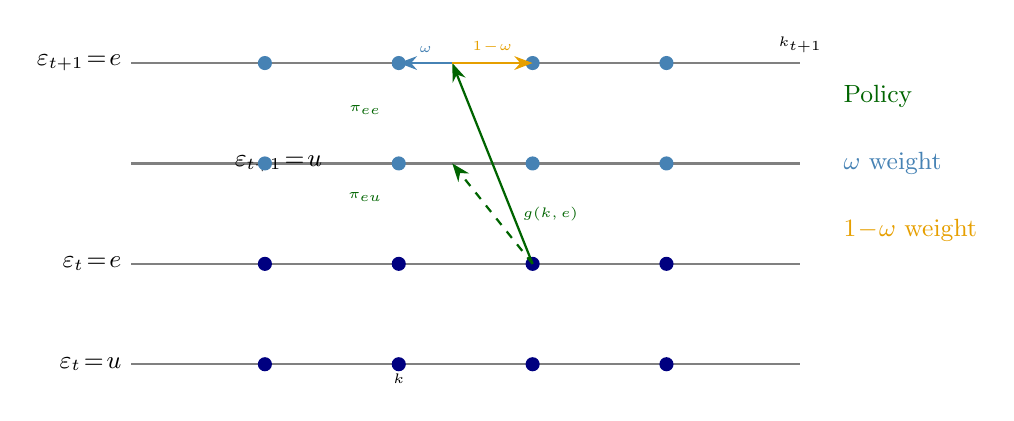
\begin{tikzpicture}[scale=0.85]
    % Grid lines
    \draw[thick, gray] (0,4.5) -- (10,4.5);
    \draw[thick, gray] (0,3) -- (10,3);
    \draw[thick, gray] (0,1.5) -- (10,1.5);
    \draw[thick, gray] (0,0) -- (10,0);

    % Labels
    \node[left, font=\small] at (0,4.5) {$\varepsilon_{t+1}\!=\!e$};
    \node[left, font=\small] at (3,3) {$\varepsilon_{t+1}\!=\!u$};
    \node[left, font=\small] at (0,1.5) {$\varepsilon_t\!=\!e$};
    \node[left, font=\small] at (0,0) {$\varepsilon_t\!=\!u$};

    % Grid points on t row
    \foreach \x in {2,4,6,8} {
        \fill[uzhblue] (\x,1.5) circle (3pt);
        \fill[uzhblue] (\x,0) circle (3pt);
    }
    % Grid points on t+1 row
    \foreach \x in {2,4,6,8} {
        \fill[softblue] (\x,4.5) circle (3pt);
        \fill[softblue] (\x,3) circle (3pt);
    }

    \node[below, font=\tiny] at (4,0) {$k$};
    \node[above, font=\tiny] at (10,4.5) {$k_{t+1}$};

    % Policy arrows from (k, e) - goes to position between grid points
    \draw[-{Stealth}, thick, darkgreen] (6,1.5) -- (4.8,4.5)
        node[near start, right, font=\tiny] {$g(k,e)$};
    \draw[-{Stealth}, thick, darkgreen, dashed] (6,1.5) -- (4.8,3);

    % Mass redistribution
    \draw[-{Stealth}, thick, softblue] (4.8,4.5) -- (4,4.5)
        node[midway, above, font=\tiny] {$\omega$};
    \draw[-{Stealth}, thick, softorange] (4.8,4.5) -- (6,4.5)
        node[midway, above, font=\tiny] {$1\!-\!\omega$};

    % Transition probabilities
    \node[font=\tiny, darkgreen] at (3.5,3.8) {$\pi_{ee}$};
    \node[font=\tiny, darkgreen] at (3.5,2.5) {$\pi_{eu}$};

    % Legend
    \node[right, font=\small] at (10.5,4) {\textcolor{darkgreen}{Policy}};
    \node[right, font=\small] at (10.5,3) {\textcolor{softblue}{$\omega$ weight}};
    \node[right, font=\small] at (10.5,2) {\textcolor{softorange}{$1\!-\!\omega$ weight}};
\end{tikzpicture}
\end{center}

{\small Arrows show: (1) policy maps current $(k,\varepsilon)$ to $k'$, (2) $k'$ is split between grid points with weight $\omega$, (3) mass transitions across $\varepsilon'$ states with probabilities $\pi_{\varepsilon'|\varepsilon}$.}
\end{frame}

% --- Slide 27a: Before/After Histogram ---
\begin{frame}{One Forward Step: Before and After}
\begin{columns}[T]
\column{0.48\textwidth}
\begin{center}
\textbf{Before:} $G_t$\\[4pt]
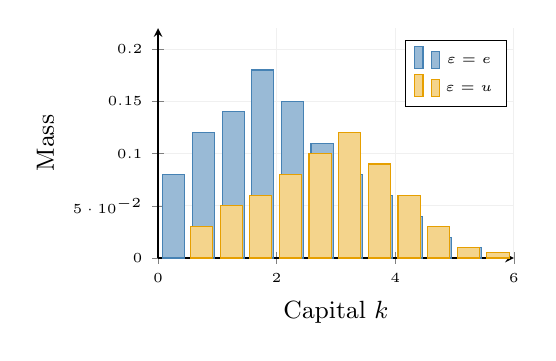
\begin{tikzpicture}
\begin{axis}[
    width=6.1cm, height=4.5cm,
    ybar, bar width=8pt,
    xlabel={Capital $k$}, ylabel={Mass},
    xlabel style={font=\small}, ylabel style={font=\small},
    tick label style={font=\tiny},
    xmin=0, xmax=6, ymin=0, ymax=0.22,
    axis lines=left,
    grid=major, grid style={gray!12},
    legend style={font=\tiny, at={(0.98,0.95)}, anchor=north east},
]
    \addplot[fill=softblue!55, draw=softblue] coordinates {
        (0.5,0.08) (1.0,0.12) (1.5,0.14) (2.0,0.18) (2.5,0.15)
        (3.0,0.11) (3.5,0.08) (4.0,0.06) (4.5,0.04) (5.0,0.02) (5.5,0.01)
    };
    \addlegendentry{$\varepsilon=e$}
    \addplot[fill=softorange!45, draw=softorange] coordinates {
        (0.5,0.03) (1.0,0.05) (1.5,0.06) (2.0,0.08) (2.5,0.10)
        (3.0,0.12) (3.5,0.09) (4.0,0.06) (4.5,0.03) (5.0,0.01) (5.5,0.005)
    };
    \addlegendentry{$\varepsilon=u$}
\end{axis}
\end{tikzpicture}\\
{\tiny Mass concentrated at low $k$; borrowing-constrained agents at left edge}
\end{center}

\column{0.48\textwidth}
\begin{center}
\textbf{After:} $G_{t+1}$\\[4pt]
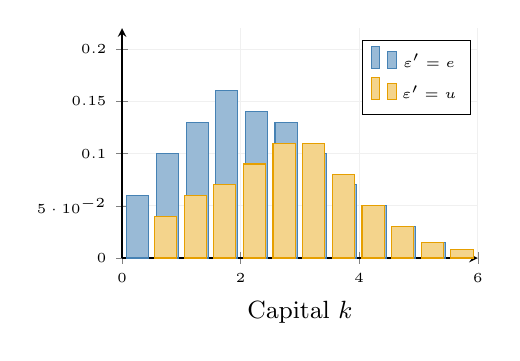
\begin{tikzpicture}
\begin{axis}[
    width=6.1cm, height=4.5cm,
    ybar, bar width=8pt,
    xlabel={Capital $k$}, ylabel={},
    xlabel style={font=\small},
    tick label style={font=\tiny},
    xmin=0, xmax=6, ymin=0, ymax=0.22,
    axis lines=left,
    grid=major, grid style={gray!12},
    legend style={font=\tiny, at={(0.98,0.95)}, anchor=north east},
]
    \addplot[fill=softblue!55, draw=softblue] coordinates {
        (0.5,0.06) (1.0,0.10) (1.5,0.13) (2.0,0.16) (2.5,0.14)
        (3.0,0.13) (3.5,0.10) (4.0,0.07) (4.5,0.05) (5.0,0.03) (5.5,0.015)
    };
    \addlegendentry{$\varepsilon'=e$}
    \addplot[fill=softorange!45, draw=softorange] coordinates {
        (0.5,0.04) (1.0,0.06) (1.5,0.07) (2.0,0.09) (2.5,0.11)
        (3.0,0.11) (3.5,0.08) (4.0,0.05) (4.5,0.03) (5.0,0.015) (5.5,0.008)
    };
    \addlegendentry{$\varepsilon'=u$}
\end{axis}
\end{tikzpicture}\\
{\tiny After policy + interpolation + shock transitions: mass slightly rightward}
\end{center}
\end{columns}

\vspace{0.3em}
\begin{center}
\tiny
Mean preserved: $\bar{k}_t = \bar{k}_{t+1}$\\[1pt]
\emphc{Exact mean preservation!}
\end{center}
\end{frame}

% --- Slide 28: Summary of Young's Method ---
\begin{frame}{Summary of Young's Method}
\begin{block}{Key Takeaways}
\begin{enumerate}
    \item Represents the distribution as a \emphc{histogram} on a fixed grid
    \item Updates \emphc{deterministically} using policy functions + transition probabilities
    \item Preserves the \emphc{mean exactly}; approximates higher moments
    \item \emphc{No sampling noise}---faster and more accurate than Monte Carlo
    \item Compatible with \emphc{any} solution method for the household problem (VFI, neural nets, \ldots)
\end{enumerate}
\end{block}

\vspace{0.5em}
\begin{center}
{\small ``Rather than use Monte Carlo simulation to generate an updated cross-sectional distribution \ldots\ I use a histogram over a fixed grid to construct tomorrow's distribution.''\\
--- Young (2010, p.~38)}
\end{center}
\end{frame}

% ============================================================================
% PART III: THE KRUSELL-SMITH ECONOMY
% ============================================================================

% --- Slide 30: Section Divider ---
\begin{frame}{}
\vfill
\begin{center}
{\Huge \textcolor{uzhblue}{\textbf{Part III}}}\\[12pt]
{\LARGE Benchmark: Krusell--Smith Logic}
\end{center}
\vfill
\end{frame}

% --- Slide 31: Model Overview ---
\begin{frame}{Benchmark: Krusell--Smith Logic}
\textbf{The Krusell--Smith (1998) economy:}

\vspace{0.5em}
\begin{itemize}
    \item \emphc{Continuum} of ex ante identical, infinitely-lived agents
    \item \emphc{Incomplete markets}: no insurance against idiosyncratic risk
    \item \emphc{Aggregate uncertainty}: productivity shocks affect all agents
    \item \emphc{Single asset}: one-period bonds/capital with borrowing constraint
\end{itemize}

\vspace{0.5em}
\begin{block}{The challenge}
Each agent must forecast future prices to make optimal savings decisions. But prices depend on the \emphc{entire wealth distribution}---which is an infinite-dimensional object.
\end{block}

\vspace{0.3em}
$\Rightarrow$ Agents use a simple forecasting rule based on the \emphc{mean} of the distribution.
\end{frame}

% --- Slide 32: Model Switch ---
\begin{frame}{Model Switch: Benchmark vs.\ Teaching Implementation}
\footnotesize
\begin{columns}[T]
\column{0.48\textwidth}
\begin{block}{Benchmark layer}
\begin{itemize}\itemsep1pt
    \item \textbf{Story model:} Krusell--Smith (1998)
    \item \textbf{Role here:} motivate approximate aggregation and the outer forecast loop
    \item \textbf{Young step:} deterministic distribution propagation inside KS
\end{itemize}
\end{block}

\column{0.48\textwidth}
\begin{block}{Teaching-code layer}
\begin{itemize}\itemsep1pt
    \item \textbf{Notebook 11:} Appendix A.5 endowment economy
    \item \textbf{Role here:} show Young's histogram as a DEQN state and simulator
    \item \textbf{Key change:} a price net replaces KS forecast-rule regression
\end{itemize}
\end{block}
\end{columns}

\vspace{0.25em}
\begin{alertblock}{Same operator, different shell}
KS explains \emphc{why} distribution tracking matters. Appendix A.5 shows the same histogram update \emphc{inside} a DEQN.
\end{alertblock}
\end{frame}

% --- Slide 33: Preferences ---
\begin{frame}{Teaching Model: Preferences}
\textbf{Epstein--Zin recursive utility} (separates risk aversion from IES):
\[
\boxed{V(x_t) = \max_{b_{t+1} \geq 0} \left[(1-\beta)\, c_t^{1-\rho} + \beta\, \chi_t\!\left(V(x_{t+1})\right)^{1-\rho}\right]^{\frac{1}{1-\rho}}}
\]

\vspace{0.3em}
\textbf{Certainty equivalent:}
\[
\chi_t(V_{t+1}) = \E{V_{t+1}^{1-\sigma}}^{\!\frac{1}{1-\sigma}}
\]

\vspace{0.3em}
\begin{center}
\begin{tabular}{lll}
\toprule
\textbf{Parameter} & \textbf{Symbol} & \textbf{Value} \\
\midrule
Discount factor & $\beta$ & 0.95 \\
Inverse of IES & $\rho$ & 2 ~~(IES $= 0.5$) \\
Risk aversion & $\sigma$ & 8 \\
\bottomrule
\end{tabular}
\end{center}

\vspace{0.2em}
{\small Note: $\rho \neq \sigma$ $\Rightarrow$ agents' intertemporal substitution and risk preferences are \emphc{separated}.}
\end{frame}

% --- Slide 34: Technology and Budget ---
\begin{frame}{Teaching Model: Budget and Shocks}
\textbf{Endowment economy} (as in Azinovic et al.\ 2022, Appendix A.5):
\begin{itemize}
    \item Aggregate output: $Y_t = w(a_t)$ depends on aggregate shock $a_t$
    \item Idiosyncratic labor endowment: $\eta_t \in \{0.8, 1.2\}$ with transition matrix $\Pi_\eta$
    \item Aggregate shocks: 6 states ($2$ uncertainty $\times$ $3$ income levels)
\end{itemize}

\vspace{0.5em}
\textbf{Budget constraint:}
\[
\boxed{c_t + p_t \cdot b_{t+1} = b_t + \eta_t \cdot w(a_t)}
\]

\vspace{0.3em}
\begin{itemize}
    \item $b_t$: bond holdings (asset)
    \item $p_t$: bond price (endogenous, clears the market)
    \item $\eta_t \cdot w(a_t)$: individual labor income
    \item \emphc{Borrowing constraint}: $b_{t+1} \geq 0$
\end{itemize}
\end{frame}

% --- Slide 35: Individual Problem ---
\begin{frame}{Teaching Model: Individual Problem}
Each agent solves:
\[
V(b, \eta, x^{agg}) = \max_{b' \geq 0} \left[(1-\beta)\, c^{1-\rho} + \beta\, \chi\!\left(V(b', \eta', x'^{agg})\right)^{1-\rho}\right]^{\frac{1}{1-\rho}}
\]

subject to:
\[
c = b + \eta \cdot w(a) - p \cdot b'
\]

\vspace{0.3em}
\textbf{State variables:}
\begin{columns}[T]
\column{0.48\textwidth}
\textbf{Individual:}
\begin{itemize}
    \item $b_t$: current bond holdings
    \item $\eta_t \in \{0.8, 1.2\}$: idiosyncratic shock
\end{itemize}

\column{0.48\textwidth}
\textbf{Aggregate:}
\begin{itemize}
    \item $a_t \in \{1, \ldots, 6\}$: aggregate shock
    \item $\mu_t$: wealth distribution (histogram)
\end{itemize}
\end{columns}

\vspace{0.3em}
{\small The bond price $p_t$ clears the market: $\int b_{t+1} \, d\mu_t = \bar B$; the teaching notebook normalizes $\bar B=1$ (unit net supply).}
\end{frame}

% --- Slide 36: Equilibrium ---
\begin{frame}{Teaching Model: Equilibrium Objects}
\begin{block}{Recursive Competitive Equilibrium}
\begin{enumerate}
    \item \textbf{Agents optimize:} given bond prices, each agent chooses $b'$ to maximize utility
    \item \textbf{Market clearing:}
    \[
    \int b_{t+1}(b, \eta, x^{agg}) \, d\mu_t(b, \eta) = \bar B,\qquad \bar B=1\ \text{in the notebook}
    \]
    \item \textbf{Distribution evolves consistently:} $\mu_{t+1} = T(\mu_t, a_t)$ given optimal policies
    \item \textbf{Rational expectations:} agents' forecast of future prices is self-confirming
\end{enumerate}
\end{block}

\vspace{0.5em}
\textbf{The bond price $p_t$:}
\begin{itemize}
    \item Depends on the aggregate state $(a_t, \mu_t)$
    \item Must be found such that aggregate demand $=$ aggregate supply $=$ 1
    \item In the DEQN approach: a \emphc{neural network} outputs $p_t$ directly
\end{itemize}
\end{frame}

% --- Slide 37: Traditional Solution Method ---
\begin{frame}{Traditional KS Solution Method}
\textbf{Step-by-step algorithm:}
\begin{enumerate}
    \item \textbf{Guess} forecasting rule: $p(a) \approx f(m_1, a)$
    \item \textbf{Solve} household problem via VFI on $(b, \varepsilon, m_1, a)$ grid
    \item \textbf{Forward-simulate} distribution via Young's method for $T$ periods
    \item \textbf{Compute} realized $m_1$ and prices from simulated distributions
    \item \textbf{Re-estimate} forecasting rule by regression on simulated data
    \item \textbf{Check convergence}: if not converged, go to step 2
\end{enumerate}

\vspace{0.5em}
\textbf{Limitations:}
\begin{itemize}
    \item VFI on fixed grid: limited resolution, curse of dimensionality
    \item Forecasting rule: restricted to low-order polynomial form
    \item Adding more moments/states is expensive
\end{itemize}

\vspace{0.3em}
$\Rightarrow$ \emphc{Can we do better with deep learning?}
\end{frame}

% --- Slide 38: KS Equilibrium Loop ---
\begin{frame}{The Krusell--Smith Outer Loop}
\begin{center}
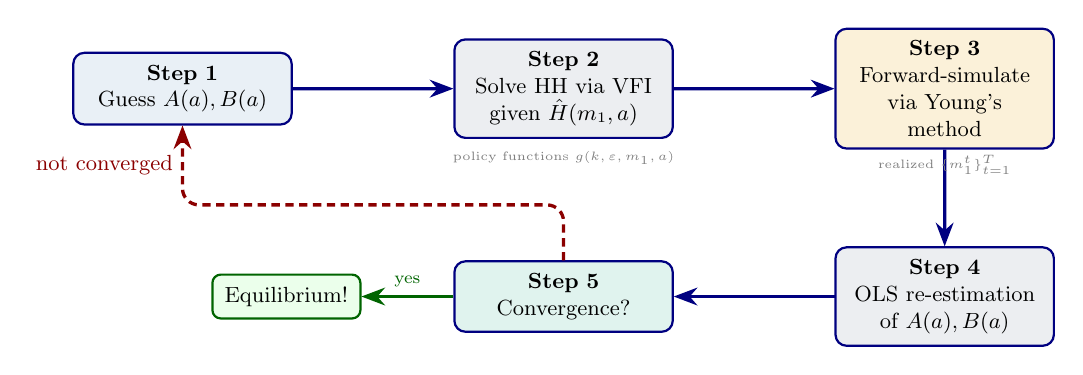
\begin{tikzpicture}[scale=0.88, every node/.style={transform shape},
    box/.style={rectangle, draw=uzhblue, thick, fill=uzhgreylight,
        minimum width=3.0cm, minimum height=1.0cm, font=\small,
        rounded corners=4pt, inner sep=5pt, text width=2.8cm, align=center},
    arr/.style={-{Stealth[length=3mm]}, thick, uzhblue, line width=1.2pt}
]
    % Nodes in a loop
    \node[box, fill=softblue!12] (guess) at (0,2.5)
        {\textbf{Step 1}\\Guess $A(a), B(a)$};
    \node[box] (vfi) at (5.5,2.5)
        {\textbf{Step 2}\\Solve HH via VFI\\given $\hat{H}(m_1,a)$};
    \node[box, fill=softorange!15] (young) at (11,2.5)
        {\textbf{Step 3}\\Forward-simulate\\via Young's method};
    \node[box] (ols) at (11,-0.5)
        {\textbf{Step 4}\\OLS re-estimation\\of $A(a), B(a)$};
    \node[box, fill=softgreen!12] (check) at (5.5,-0.5)
        {\textbf{Step 5}\\Convergence?};

    % Arrows
    \draw[arr] (guess) -- (vfi);
    \draw[arr] (vfi) -- (young);
    \draw[arr] (young) -- (ols);
    \draw[arr] (ols) -- (check);

    % Loop back if not converged
    \draw[arr, darkred, densely dashed, rounded corners=6pt]
        (check.north) -- ++(0,0.8) -- ++(-5.5,0) -- (guess.south)
        node[midway, left, font=\small, darkred] {not converged};

    % Done
    \node[rectangle, draw=darkgreen, thick, fill=green!8, rounded corners=3pt,
        inner sep=5pt, font=\small] (done) at (1.5,-0.5) {Equilibrium!};
    \draw[arr, darkgreen] (check.west) -- (done.east)
        node[midway, above, font=\scriptsize, darkgreen] {yes};

    % Annotations
    \node[font=\tiny, gray] at (5.5,1.5) {policy functions $g(k,\varepsilon,m_1,a)$};
    \node[font=\tiny, gray] at (11,1.4) {realized $\{m_1^t\}_{t=1}^T$};
\end{tikzpicture}
\end{center}

\vspace{0.2em}
{\small Young's simulation makes the forward-distribution step deterministic and fast, but total runtime still depends on the VFI tolerance, forecasting-rule tolerance, and implementation.}
\end{frame}

% ============================================================================
% PART IV: DEQN IMPLEMENTATION
% ============================================================================


\end{document}
